\section{方法}
本研究で開発したmy\_helpからhikiへの自動変換ソフトmy\_help2hiki
はmy\_helpのgemに組み込んでいる.
本章では,my\_help2hikiのコマンドとコマンドによる振る舞いを記述する.

\begin{figure}[htbp]\begin{center}
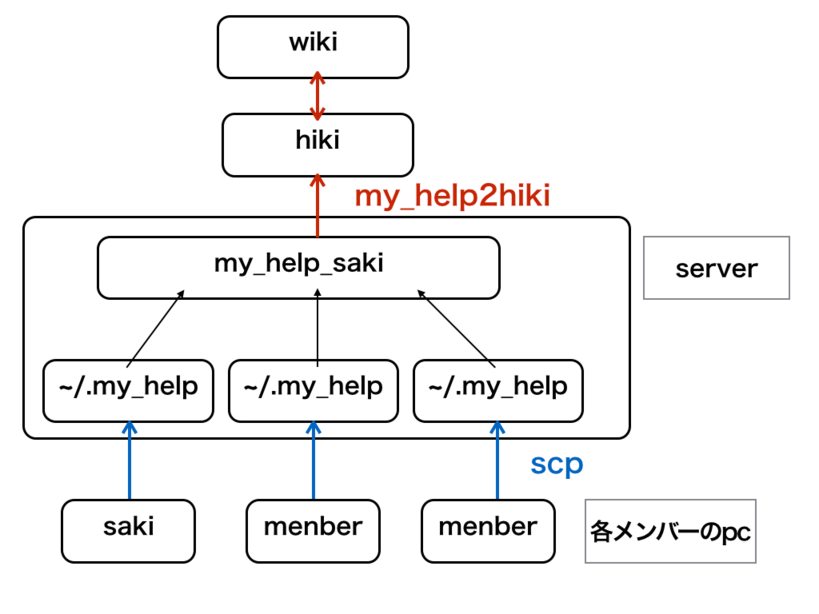
\includegraphics[width=6cm,bb=100 100 600 700]{my_help2hiki_saki.010.png}
\caption{my\_help2hiki}
\label{default}\end{center}\end{figure}

\begin{description}
\item my
my\_help2hikiは図のようになっている,
各学生がmy\_helpで作ったメモは.my\_helpのディレクトリに保存される.
これをscpコマンドを利用してserverのmy\_help\_sakiのディレクトリにコピーする.
コピーしたmy\_helpの内容をmy\_help2hikiを利用してhikiに変換し,wikiで表示する.
\end{description}

\subsection{my\_help/lib/specific\_help.rb}
\begin{description}
\item specific\_help.rbは以下のようになっている
\end{description}
\begin{quote}\begin{verbatim}
/Users/saki/my_help/lib% cat specific_help.rb
# -*- coding: utf-8 -*-
require "optparse"
require "yaml"
require "my_help/version"
require 'fileutils'
require "coderay"

module SpecificHelp
  class Command

    def self.run(file,argv=[])
      new(file, argv).execute
    end

    def initialize(file,argv=[])
      @source_file = file
      @help_cont = YAML.load(File.read(file))
      @help_cont[:head].each{|line| print line.chomp+"\n" } if @help_cont[:head] != nil
      @help_cont[:license].each{|line| print "#{line.chomp}\n" } if @help_cont[:license] != nil
      @argv = argv
    end

    def execute
      if @argv.size==0
        if @source_file.include?('todo')
          @argv << '--all'
        else
          @argv << '--help'
        end
      end
      command_parser = OptionParser.new do |opt|
        opt.on('-v', '--version','show program Version.') { |v|
          opt.version = MyHelp::VERSION
          puts opt.ver
        }
        @help_cont.each_pair{|key,val|
          next if key==:head or key==:license
          opts = val[:opts]
          opt.on(opts[:short],opts[:long],opts[:desc]) {disp_help(key)}
        }
        opt.on('--edit','edit help contents'){edit_help}
        opt.on('--to_hiki','convert to hikidoc format'){to_hiki}
        opt.on('--all','display all helps'){all_help}
        opt.on('--store [item]','store [item] in backfile'){|item| store(item)}
        opt.on('--push', 'push my_todo on remote host'){push}
        opt.on('--remove [item]','remove [item] and store in backfile'){|item| remove(item) }
        opt.on('--add [item]','add new [item]'){|item| add(item) }
        opt.on('--backup_list [val]','show last [val] backup list'){|val| backup_list(val)}
      end
      begin
        command_parser.parse!(@argv)
      rescue=> eval
        p eval
      end
      exit
    end

    def backup_list(val)
      val = val || 10
      print "\n ...showing last #{val} stored items in backup.\n"
      backup=mk_backup_file(@source_file)
      File.open(backup,'r'){|file|
        backup_cont = YAML.load(File.read(backup))
        backup_size = backup_cont.size
        backup_size = backup_size>val.to_i ? val.to_i : backup_size
        backup_keys = backup_cont.keys
        backup_keys.reverse.each_with_index{|item,i|
          break if i>=backup_size
          line = item.to_s.split('_')
          printf("%10s : %8s%8s\n",line[0],line[1],line[2])
        }
      }
    end

    def mk_backup_file(file)
      path = File.dirname(file)
      base = File.basename(file)
      backup= File.join(path,"."+base)
      FileUtils.touch(backup) unless File.exists?(backup)
      return backup
    end

    def store(item)
      if item==nil
        print "spcify --store [item].\n"
        exit
      else
        print "Trying to store #{item}\n"
      end
      backup=mk_backup_file(@source_file)
      unless store_item = @help_cont[item.to_sym] then
        print "No #{item} in this help.  The items are following...\n"
        keys = @help_cont.keys
        keys.each{|key|
          p key
        }
        exit
      end
      p store_name = item+"_"+Time.now.strftime("%Y%m%d_%H%M%S")
      backup_cont=YAML.load(File.read(backup)) || {}
      backup_cont[store_name.to_sym]=store_item
      File.open(backup,'w'){|file| file.print(YAML.dump(backup_cont))}
    end


    def push
      p "push my_todo"
      data_dir = File.join(ENV['HOME'],'.my_help')
      FileUtils.cd(data_dir)
      system "pwd"
      system "rm -rf ~/.my_help/*.yml~"
      system "scp -r ~/.my_help saki@nishitani0:~"
      system "ssh saki@nishitani0 ls ~/.my_help" 


    end


    def add(item='new_item')
      print "Trying to add #{item}\n"
      new_item={:opts=>{:short=>'-'+item[0], :long=>'--'+item, :desc=>item},
          :title=>item, :cont=> [item]}
      @help_cont[item.to_sym]=new_item
      File.open(@source_file,'w'){|file| file.print YAML.dump(@help_cont)}    end

    def remove(item)
      print "Trying to remove #{item}\n"
      store(item)
      @help_cont.delete(item.to_sym)
      File.open(@source_file,'w'){|file| file.print YAML.dump(@help_cont)}
    end

    def edit_help
      system("emacs #{@source_file}")
    end

    def to_hiki
      @help_cont.each_pair{|key,val|
        if key==:head or key==:license
          hiki_disp(val)
        else
          hiki_help(key)
        end
      }
    end

    def all_help
      @help_cont.each_pair{|key,val|
        if key==:head or key==:license
          val[0]+=":"
          disp(val)
        else
          disp_help(key)
        end
      }
    end

    def hiki_help(key_word)
      items =@help_cont[key_word]
      puts "\n!!"+items[:title]+"\n"
      hiki_disp(items[:cont])
    end

    def hiki_disp(lines)
      lines.each{|line| puts "*#{line}"}  if lines != nil
    end

    def disp_help(key_word)
      print_separater
      items =@help_cont[key_word]
      puts CodeRay.scan("-#{items[:title]}:", :Taskpaper).term
      disp(items[:cont])
      print_separater
    end

    def disp(lines)
      lines.each{|line| puts CodeRay.scan("+#{line}", :Taskpaper).term}
    end

    def print_separater
      print "---\n"
    end
    
  end
end
\end{verbatim}\end{quote}

\subsection{my\_help/lib/my\_help.rb}
\begin{description}
\item my\_help.rbは以下のようになっている.
\end{description}
\begin{quote}\begin{verbatim}
/Users/saki/my_help/lib% cat my_help.rb
# -*- coding: utf-8 -*-
require "optparse"
require "yaml"
require "fileutils"
require "my_help/version"
require "systemu"

module MyHelp
  class Command

    def self.run(argv=[])
      new(argv).execute
    end

    def initialize(argv=[])
      @argv = argv
      @default_help_dir = File.expand_path("../../lib/daddygongon", __FILE__)
      @local_help_dir = File.join(ENV['HOME'],'.my_help')
      set_help_dir_if_not_exists
    end

    def set_help_dir_if_not_exists
      return if File::exists?(@local_help_dir)
      FileUtils.mkdir_p(@local_help_dir, :verbose=>true)
      Dir.entries(@default_help_dir).each{|file|
        next if file=='template_help.yml'
        file_path=File.join(@local_help_dir,file)
        next if File::exists?(file_path)
        FileUtils.cp((File.join(@default_help_dir,file)),@local_help_dir,:verbose=>true)
      }
    end

    def execute
      @argv << '--help' if @argv.size==0
      command_parser = OptionParser.new do |opt|
        opt.on('-v', '--version','show program Version.') { |v|
          opt.version = MyHelp::VERSION
          puts opt.ver
        }
        opt.on('-l', '--list', 'list specific helps'){list_helps}
        opt.on('-e NAME', '--edit NAME', 'edit NAME help(eg test_help)'){|file| edit_help(file)}
        opt.on('-i NAME', '--init NAME', 'initialize NAME help(eg test_help).'){|file| init_help(file)}
        opt.on('-m', '--make', 'make executables for all helps.'){make_help}
        opt.on('-c', '--clean', 'clean up exe dir.'){clean_exe}
        opt.on('--install_local','install local after edit helps'){install_local}
        opt.on('--delete NAME','delete NAME help'){|file| delete_help(file)}
        opt.on('--hiki','my_help2hiki'){hiki}
      end
      begin
        command_parser.parse!(@argv)
      rescue=> eval
        p eval
      end
      exit
    end

    def delete_help(file)
      del_files=[]
      del_files << File.join(@local_help_dir,file)
       exe_dir=File.join(File.expand_path('../..',@default_help_dir),'exe')
       del_files << File.join(exe_dir,file)
      p del_files << File.join(exe_dir,short_name(file))
      print "Are you sure to delete these files?[yes]"
      if gets.chomp=='yes' then
        del_files.each{|file| FileUtils.rm(file,:verbose=>true)}
      end
    end

    USER_INST_DIR="USER INSTALLATION DIRECTORY:"
    INST_DIR="INSTALLATION DIRECTORY:"
    def install_local
      Dir.chdir(File.expand_path('../..',@default_help_dir))
      p pwd_dir = Dir.pwd
      status, stdout, stderr = systemu "gem env|grep '#{USER_INST_DIR}'"
      if stdout==""
        status, stdout, stderr = systemu "gem env|grep '#{INST_DIR}'"
      end
      p system_inst_dir = stdout.split(': ')[1].chomp
      if pwd_dir == system_inst_dir
        puts "Download my_help from github, and using bundle for edit helps\n"
        puts "Read README in detail.\n"
        exit
      end
      system "git add -A"
      system "git commit -m 'update exe dirs'"
      system "Rake install:local"
    end

    def short_name(file)
      file_name=file.split('_')
      return file_name[0][0]+"_"+file_name[1][0]
    end

    def make_help
      local_help_entries.each{|file|
        exe_cont="#!/usr/bin/env ruby\nrequire 'specific_help'\n"
        exe_cont << "help_file = File.join(ENV['HOME'],'.my_help','#{file}')\n"
        exe_cont << "SpecificHelp::Command.run(help_file, ARGV)\n"
        file = File.basename(file,'.yml')
        [file, short_name(file)].each{|name|
          p target=File.join('exe',name)
          File.open(target,'w'){|file| file.print exe_cont}
          FileUtils.chmod('a+x', target, :verbose => true)
        }
      }
      install_local
    end

    def clean_exe
      local_help_entries.each{|file|
        next if ['emacs_help','e_h','my_help','my_todo'].include?(file)
        file = File.basename(file,'.yml')
        [file, short_name(file)].each{|name|
          p target=File.join('exe',name)
          FileUtils::Verbose.rm(target)
        }
      }
    end

    def init_help(file)
      p target_help=File.join(@local_help_dir,file+'.yml')
      if File::exists?(target_help)
        puts "File exists. rm it first to initialize it."
        exit
      end
      p template = File.join(@default_help_dir,'template_help.yml')
      FileUtils::Verbose.cp(template,target_help)
    end

    def edit_help(file)
      p target_help=File.join(@local_help_dir,file)
      system "emacs #{target_help}.yml"
    end

    def local_help_entries
      entries= []
      Dir.entries(@local_help_dir).each{|file|
        next unless file.include?('_')
        next if file[0]=='#' or file[-1]=='~' or file[0]=='.'
        entries << file
      }
      return entries
    end

    def list_helps
      print "Specific help file:\n"
      local_help_entries.each{|file|
        file_path=File.join(@local_help_dir,file)
        file = File.basename(file,'.yml')
        begin
          help = YAML.load(File.read(file_path))
        rescue=> eval
          p eval
          print "\n YAML load error in #{file}."
          print "  See the line shown above and revise by\n"
          print "  emacs #{file_path}\n"
          exit
        end
        print "  #{file}\t:#{help[:head][0]}\n"
      }
    end

    def hiki
      system "ls ~/.my_help2"
      system "emacs_help --to_hiki > ~/Sites/hiki-1.0/data/text/emacs_help_saki"
      system "my_todo --to_hiki > ~/Sites/hiki-1.0/data/text/my_todo_saki"
      system "ssh_help --to_hiki > ~/Sites/hiki-1.0/data/text/ssh_help_saki"
      system "open -a safari 'http://localhost/~saki/hiki-1.0/?FrontPage'"
    end

  end
end
\end{verbatim}\end{quote}


\subsection{使用法,コマンド}
\begin{itemize}
\item TARGET --push : 作成したメモ(TARGET)をサーバに送る
\end{itemize}  
\begin{itemize}
\item my\_help --hiki : 作成したメモをhiki形式に変換し,wikiで表示できるようにする.
\end{itemize}

\subsection{コマンドの振る舞い}
\paragraph{TARGET --push}

\begin{figure}[htbp]\begin{center}
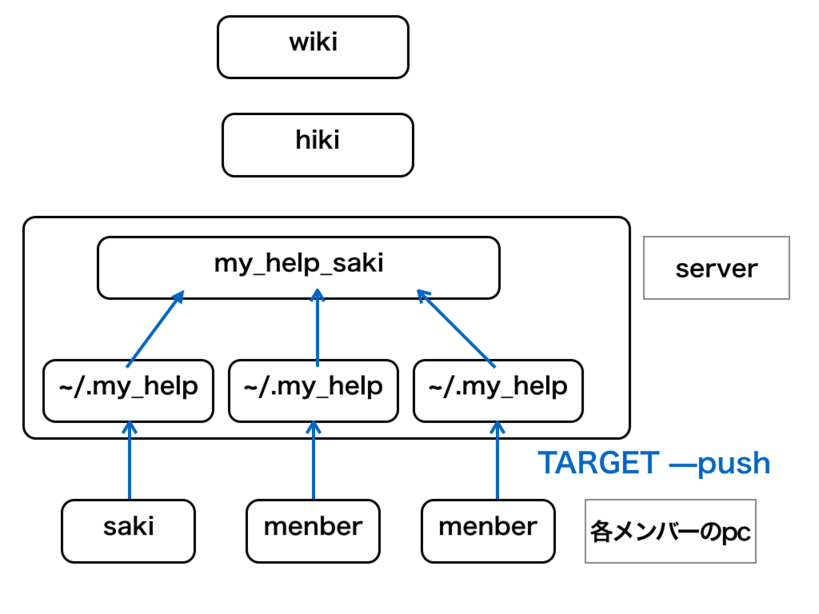
\includegraphics[width=6cm,bb=100 100 600 700]{my_help2hiki_saki.012.png}
\caption{TARGET --push}
\label{default}\end{center}\end{figure}

\begin{quote}\begin{verbatim}
    def push
      p "push my_todo"
      data_dir = File.join(ENV['HOME'],'.my_help')
      FileUtils.cd(data_dir)
      system "pwd"
      system "rm -rf ~/.my_help/*.yml~"
      system "scp -r ~/.my_help saki@nishitani0:~"
      system "ssh saki@nishitani0 ls ~/.my_help" 
\end{verbatim}\end{quote}

\begin{itemize}
\item 3,4行目
\end{itemize}
\begin{description}
\item my\_helpでは,作成したメモが.my\_helpのディレクトリに自動的に追加されるので,
ディレクトリを.my\_helpに移動する.
\end{description}
\begin{itemize}
\item 6行目
\end{itemize}
\begin{description}
\item .my\_helpにメモが追加されるとき,yaml形式のファイルで保存される.
メモを更新すると,一つ前に保存したファイルは*.yml~というファイル名
でバックアップとして残される.
\textbf{rm -rf}で不必要なファイルは削除し,サーバにコピーするときのデータ量を減らしている.
\end{description}

\begin{itemize}
\item 7行目
\end{itemize}
\begin{description}
\item
\textbf{scp -r ~/[directory名] [server名]}
serverにssh接続を行い,directoryをserverにコピーする.
-rはディレクトリ全体をコピーすることを示している.
西谷研究室で利用しているnishitani0というサーバにコピーしている.
\end{description}

\begin{itemize}
\item 8行目
\end{itemize}
\begin{description}
\item nishitani0にssh接続し.my\_helpの中身を書き出して,
コピーができているかコマンドを実行した時に確認が行えるようにしている.
\end{description}

\paragraph{my\_help --hiki}

\begin{figure}[htbp]\begin{center}
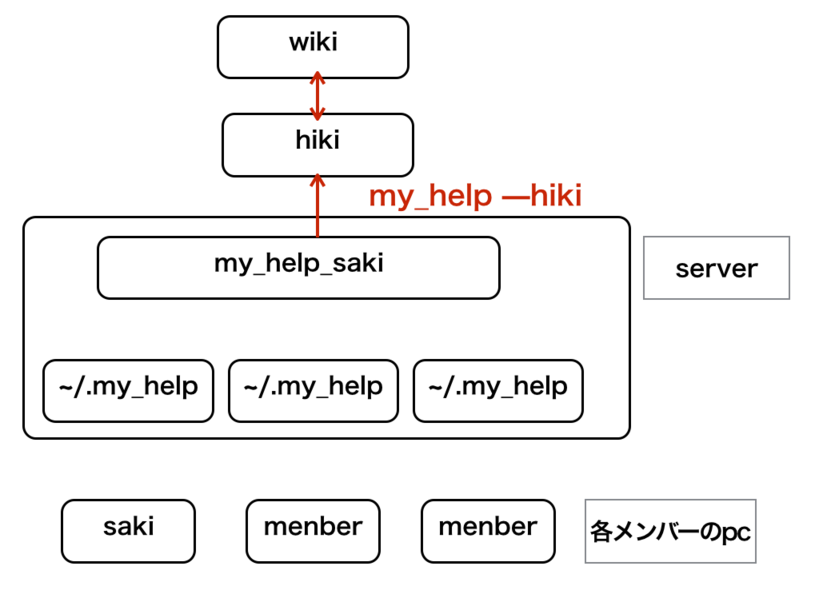
\includegraphics[width=6cm,bb=100 100 600 700]{my_help2hiki_saki.013.png}
\caption{my\_help2hiki}
\label{default}\end{center}\end{figure}


\begin{quote}\begin{verbatim}
def hiki
      p 'my_help2hiki'
      system "emacs_help --to_hiki > ~/Sites/hiki-1.0/data/text/emacs_help_saki"
      system "my_todo --to_hiki > ~/Sites/hiki-1.0/data/text/my_todo_saki"
      system "ssh_help --to_hiki > ~/Sites/hiki-1.0/data/text/ssh_help_saki"
      system "open -a safari 'http://localhost/~saki/hiki-1.0/?FrontPage'"
    end
\end{verbatim}\end{quote}
\begin{itemize}
\item 2-4行目
\end{itemize}
\begin{description}
\item my\_helpには,\textbf{TARGET --to\_hiki}というコマンドがあり,これによって
yaml形式で保存されているメモをhiki形式で書き出すことができる.
この --hiki のコマンドを使ってhiki形式にしたものを,wikiで表示することのできる
フォルダである\textbf{~/Sites/hiki-1.0/data/text/}に入れることで,wikiでの表示を可能にしている.
emacs\_help,my\_todo,ssh\_helpは全て私のmy\_helpに入っているメモ.
\end{description}

\begin{itemize}
\item 5行目
\end{itemize}
\begin{description}
\item wikiのページ図6に示したFrontPageを表示するコマンド.
これによりメモが更新されているのを即時確認することができる.
FrontPageは以下のようになっている.
\end{description}
\begin{quote}\begin{verbatim}
!saki's help
*[[ssh_help_saki]]
*[[my_todo_saki]]
*[[emacs_help_saki]]
\end{verbatim}\end{quote}
\begin{description}
\item 先頭に\textbf{!}をつけることで1行目のsaki's helpを見出しにし,
2~4行目は\textbf{*}によって箇条書き,角括弧でリンクになっている.
\end{description}

\begin{figure}[htbp]\begin{center}
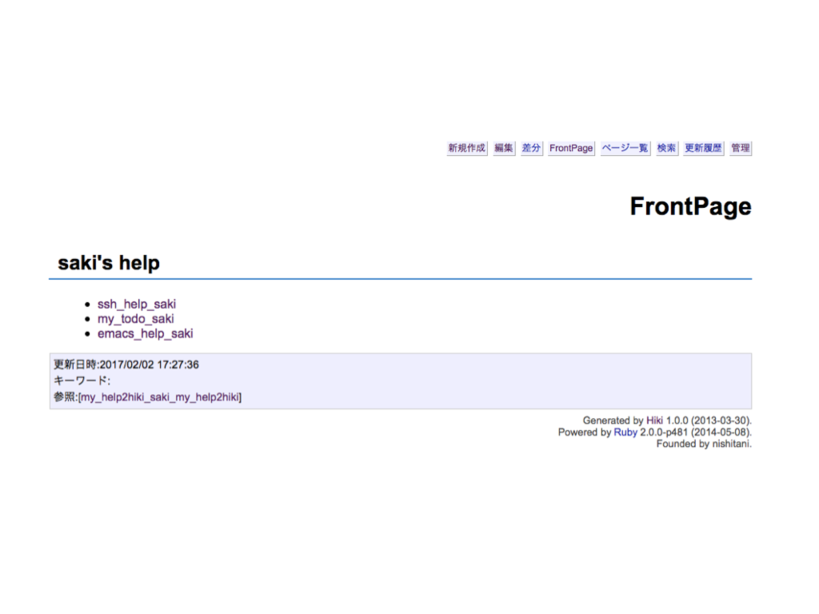
\includegraphics[width=6cm,bb=100 100 600 700]{my_help2hiki_saki.002.png}
\caption{コマンドを実行したときに開くFrontPage }
\label{default}\end{center}\end{figure}

